% !TeX root = ../../documento.tex

% \includepdf[pages=-]{lib/ABS_Valve_Board.pdf} 

% \includepdf[pages=-]{lib/PDB_Image.pdf} 

\chapter{Circuitos Propostos da Plataforma de Controle}
\label{ap:circuitos-propostos}

Este apêndice apresenta os esquemáticos completos, diagramas elétricos e simulações dos circuitos utilizados para o condicionamento de sinais, acionamento de válvulas, controle da bomba eletro-hidráulica e leitura de sensores. Esses circuitos complementam a descrição funcional apresentada na Seção~\ref{sec:metodologia-6-1}.

\section{Circuito Comparador para o Sensor de Velocidade}
\label{ap:circuito-sensor-roda}

O sinal proveniente do sensor de velocidade da roda apresenta baixa amplitude e suscetibilidade a ruído. Para seu condicionamento, adotou-se um circuito comparador baseado em amplificador operacional, garantindo níveis lógicos compatíveis com o microcontrolador.

\begin{figure}[htbp]
    \centering
    \caption{Circuito Sensor de Roda Proposto.}
    \label{fig:ap-circuito-sensor-de-roda-proposto}
    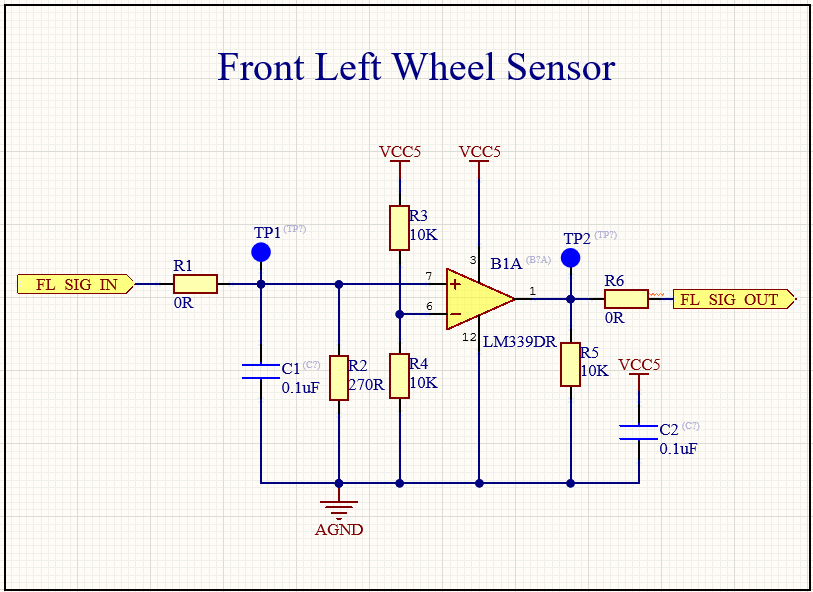
\includegraphics[width=0.8\textwidth]{figuras/circuito-sensor-de-roda-proposto.png}
\end{figure}

O comparador limitado em 2.5V permite transformar o sinal analógico variável em um nível lógico digital, operando em 3.3V para o microcontrolador. A simulação realizada no LTSpice confirma a transição correta entre níveis lógicos conforme as variações do sensor.

\begin{figure}[htbp]
    \centering
    \caption{Simulação do Circuito Sensor de Roda Proposto.}
    \label{fig:ap-simulacao-circuito-sensor-de-roda-proposto}
    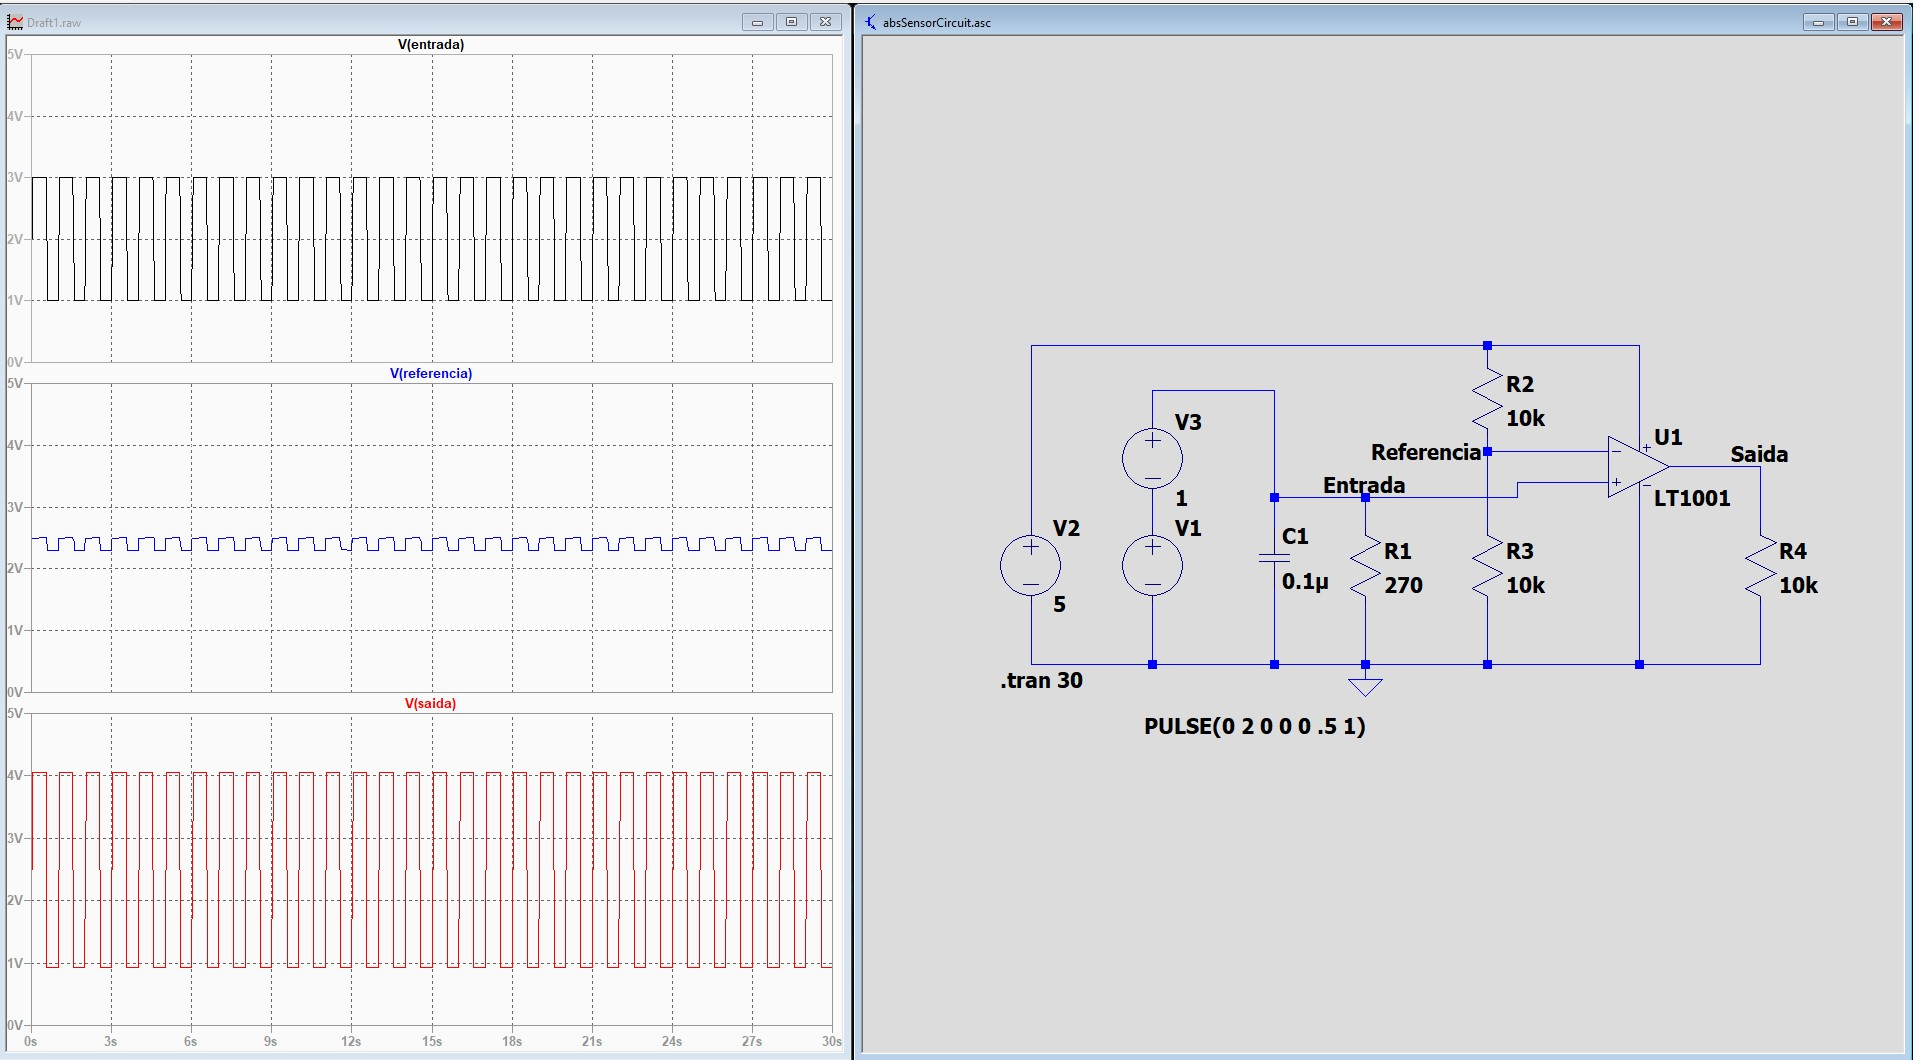
\includegraphics[width=0.8\textwidth]{figuras/simulacao-circuito-sensor-de-roda-proposto.jpg}
\end{figure}

\section{Circuito de Acionamento das Válvulas Solenoides}
\label{ap:circuito-valvulas}

O circuito das válvulas solenoides foi baseado no kit de freio NXP KITVALVECNTLEVM, utilizando os circuitos integrados MC34SB0800 e MC34SB0410, responsáveis pelo controle de múltiplas válvulas e de um motor associado.

\begin{figure}[htbp]
    \centering
    \caption{Circuito de Controle das Válvulas Solenoides.}
    \label{fig:ap-circuito-controle-valvula-solenoide}
    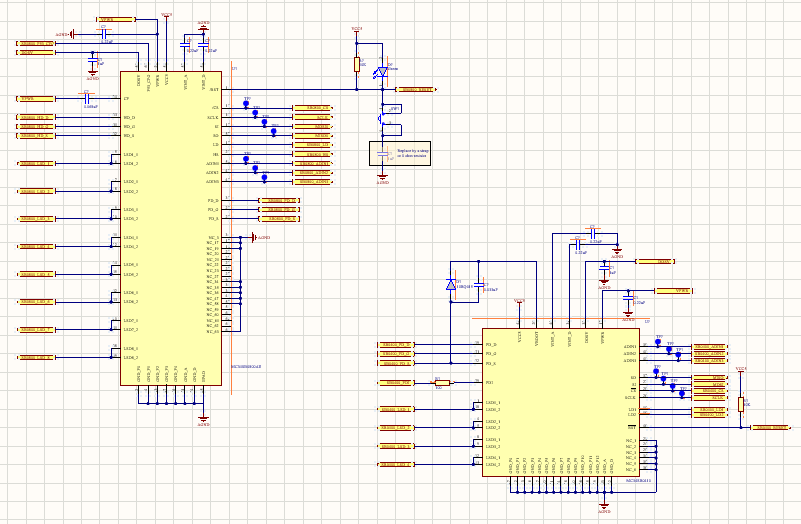
\includegraphics[width=0.8\textwidth]{figuras/circuito-controle-valvula-solenoide.png}
\end{figure}

O uso desses CIs garante proteção de corrente, controle independente das válvulas e compatibilidade com frequências de chaveamento exigidas pela aplicação automotiva.

\section{Circuito de Controle do Motor da Bomba}
\label{ap:circuito-bomba}

Para o acionamento da bomba eletro-hidráulica, o circuito foi desenvolvido com base no mesmo kit da NXP. O MC34SB0800 permite controle PWM de até 500 Hz, enquanto o MC34SB0410 opera até 16 kHz, possibilitando controle mais silencioso e preciso.

\begin{figure}[htbp]
    \centering
    \caption{Circuito de Controle da Bomba de Pressão.}
    \label{fig:ap-circuito-controle-bomba}
    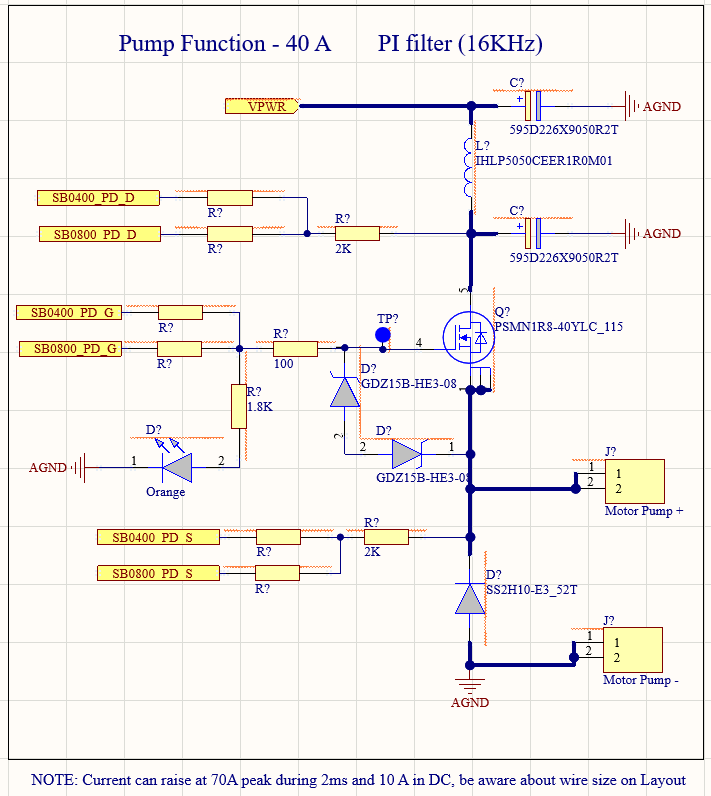
\includegraphics[width=0.8\textwidth]{figuras/circuito-controle-valvula-motor.png}
\end{figure}

Ambos os drivers incluem recursos de proteção e monitoramento essenciais para garantir a integridade do sistema.

\section{Circuito de Leitura do Sensor de Pressão}
\label{ap:circuito-pressao}

Para leitura da pressão hidráulica, selecionou-se um sensor piezoresistivo (strain gauge), devido à robustez e sensibilidade adequada ao sistema de freio. Um amplificador de instrumentação foi utilizado para garantir rejeição de ruído e amplificação precisa do sinal diferencial.

\begin{figure}[htbp]
    \centering
    \caption{Circuito de Leitura do Sensor de Pressão.}
    \label{fig:ap-circuito-sensor-de-pressao}
    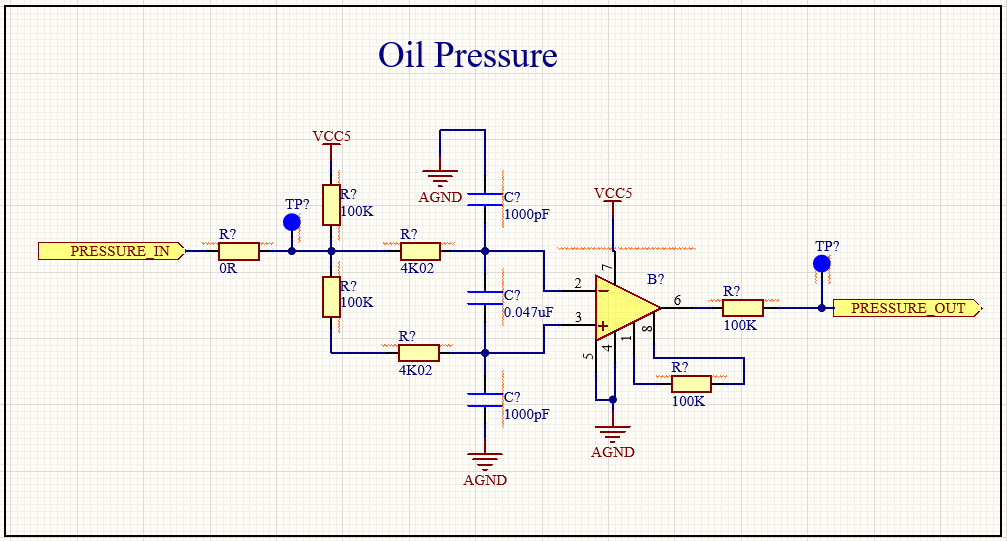
\includegraphics[width=0.8\textwidth]{figuras/circuito-sensor-de-pressao-proposto.png}
\end{figure}

O circuito condiciona o sinal do sensor para níveis adequados de leitura pelo microcontrolador, garantindo estabilidade e confiabilidade durante o processamento dos dados.








% \includepdf[pages=-]{lib/ABS_Valve_Board.pdf} 

% \includepdf[pages=-]{lib/PDB_Image.pdf} 

\section{Scripts MATLAB e Simulink Utilizados}
\label{ap:scripts-matlab}

Esta seção reúne os scripts utilizados para gerar as figuras de simulação inseridas no trabalho.

Os códigos citados no texto incluem: (i) o bloco \texttt{MATLAB Function} do modelo hidráulico 2P (Código~\ref{cod:bloco_hidraulico_2p}); (ii) o \textit{script} do ensaio integrado em malha aberta (Código~\ref{cod:ensaio_integrado_malha_aberta}); e (iii) o \textit{script} de síntese e execução do controlador LQI (Código~\ref{cod:script_controle_lqi_luenberger}), além dos códigos dos blocos de controle usados no Simulink (Códigos~\ref{cod:matlab_function_lqi_observer} e \ref{cod:matlab_function_valvulas_onoff}).


\begin{lstlisting}[caption={Bloco MATLAB Function do modelo hidráulico 2P}, label={cod:bloco_hidraulico_2p}, language=Matlab]
function [Psup_dot, Pw_dot, Qpump, Qin, Qout] = Bloco_Hidraulico_2P(omega_p, u_in, u_out, Psup, Pw)
% omega_p: rad/s (>=0)
% u_in, u_out: 0..1 (PWM normalizado / abertura proporcional)
% Psup, Pw: Pa
% Saidas: derivadas de pressao e vazoes (m^3/s)

% ---------- parametros hidraulicos basicos ----------
beta = 1.5e9;   % Pa - modulo volumetrico efetivo (oleo + mangueiras)
rho  = 850;     % kg/m^3 - densidade tipica de fluido de freio
Pret = 1e5;     % Pa - pressao de retorno (aprox. atmosferica)

% ---------- volumes efetivos ----------
Vsup = 6.0e-5;   % m^3
Vw   = 1.0e-5;   % m^3

% ---------- bomba (modelo linear simples) ----------
Dp_rev = 5e-7;                  % m^3/rev
Nv     = 0.85;                  % eficiencia volumetrica
Kb     = Nv * (Dp_rev/(2*pi));  % m^3/rad
Klb    = 1e-11;                 % (m^3/s)/Pa

% ---------- valvulas (lei do orificio) ----------
Cv_in    = 0.62;
Cv_out   = 0.62;
Ain_max  = 3.0e-7;              % m^2
Aout_max = 3.0e-7;              % m^2

% Vazamentos opcionais
Kleak_sup = 0;                  % (m^3/s)/Pa
Kleak_w   = 0;                  % (m^3/s)/Pa

% ---------- sanitizacao de entradas ----------
if omega_p < 0
    omega_p = 0;
end
u_in  = min(max(u_in,  0), 1);
u_out = min(max(u_out, 0), 1);

% Evita pressoes abaixo do retorno (numerico)
Psup = max(Psup, Pret);
Pw   = max(Pw,   Pret);

% ---------- bomba -> suprimento ----------
Qpump = Kb*omega_p - Klb*(Psup - Pret);

% ---------- suprimento -> roda (valvula de entrada) ----------
dPin = max(Psup - Pw, 0);
Qin  = Cv_in * (Ain_max * u_in) * sqrt(2*dPin/rho);

% ---------- roda -> retorno (valvula de saida) ----------
dPout = max(Pw - Pret, 0);
Qout  = Cv_out * (Aout_max * u_out) * sqrt(2*dPout/rho);

% ---------- dinamica das pressoes ----------
Psup_dot = (beta/Vsup) * ( Qpump - Qin - Kleak_sup*(Psup - Pret) );
Pw_dot   = (beta/Vw)   * ( Qin - Qout - Kleak_w*(Pw   - Pret) );
end
\end{lstlisting}

\begin{lstlisting}[caption={Script MATLAB do ensaio integrado em malha aberta}, label={cod:ensaio_integrado_malha_aberta}, language=Matlab]
%% ensaio_integrado_malha_aberta.m
% Ensaio integrado em malha aberta:
% Fase A: pressurizacao (omega_p > 0, u_in = 1, u_out = 0)
% Fase B: retencao (omega_p = 0, u_in = 0, u_out = 0)
% Fase C: alivio (omega_p = 0, u_in = 0, u_out > 0)

clear; close all; clc;

mdl = 'BlocoHidraulico';
load_system(mdl);

% Tempo total e condicoes iniciais
Tstop = 4.0;   % s
Pret  = 1e5;   % Pa
Psup0 = Pret;
Pw0   = Pret;
assignin('base','Pret',Pret);
assignin('base','Psup0',Psup0);
assignin('base','Pw0',Pw0);

% Definicao de fases no tempo:
tA_end = 2.0;
tB_end = 3.0;
tC_end = Tstop;

%% Sinal da bomba: omega_p(t)
t_omega = [0    0.5  0.5  1.5  1.5  tA_end ...
           tA_end tB_end tB_end tC_end]';
v_omega = [0    0    30   30   15   15   ...
           0     0    0    0   ]';
omega_p_ts = timeseries(v_omega, t_omega);

%% Sinal da valvula de entrada: u_in(t)
t_uin = [0    tA_end tA_end tC_end]';
v_uin = [1       1      0      0 ]';
u_in_ts = timeseries(v_uin, t_uin);

%% Sinal da valvula de saida: u_out(t)
t_uout = [0    tB_end tB_end tC_end]';
v_uout = [0       0      0.8   0.8 ]';
u_out_ts = timeseries(v_uout, t_uout);

%% Enviar para workspace do modelo
assignin('base','omega_p_ts',omega_p_ts);
assignin('base','u_in_ts',u_in_ts);
assignin('base','u_out_ts',u_out_ts);

%% Configuracao do modelo e simulacao
set_param(mdl, 'StopTime', num2str(Tstop), ...
               'Solver',   'ode15s',      ...
               'MaxStep',  '1e-4');

simOut = sim(mdl);

%% Leitura de sinais (logsout ou To Workspace)
if isprop(simOut,'logsout') && ~isempty(simOut.logsout)
    logs = simOut.logsout;
    getTS = @(name) logs.get(name).Values;
    Psup    = getTS('Psup_bar_g');
    Pw      = getTS('Pw_bar_g');
    Qpump   = getTS('Qpump_mLs');
    Qin     = getTS('Qin_mLs');
    Qout    = getTS('Qout_mLs');
    omega_p = getTS('omega_p');
    u_in    = getTS('u_in');
    u_out   = getTS('u_out');
else
    Psup    = simOut.get('Psup_bar_g');
    Pw      = simOut.get('Pw_bar_g');
    Qpump   = simOut.get('Qpump_mLs');
    Qin     = simOut.get('Qin_mLs');
    Qout    = simOut.get('Qout_mLs');
    omega_p = simOut.get('omega_p');
    u_in    = simOut.get('u_in');
    u_out   = simOut.get('u_out');
end

Psup_g_bar = Psup.Data;
Pw_g_bar   = Pw.Data;
Qpump_ml_s = Qpump.Data;
Qin_ml_s   = Qin.Data;
Qout_ml_s  = Qout.Data;

%% Configuracao de plots
set(groot,'defaultLineLineWidth',1.6);
set(groot,'defaultAxesFontSize',11);
set(groot,'defaultAxesFontName','Times New Roman');

fig = figure('Color','w','Position',[100 100 980 720]);
tiledlayout(3,1,'TileSpacing','compact','Padding','compact');

% Entradas
nexttile;
plot(omega_p.Time, omega_p.Data,'k'); hold on;
plot(u_in.Time,  u_in.Data*max(omega_p.Data),'b--');
plot(u_out.Time, u_out.Data*max(omega_p.Data),'r--');
grid on; ylabel('\\omega_p (rad/s)');
title('Entradas');
legend('\\omega_p','u_{in} (esc.)','u_{out} (esc.)','Location','best');
ymax = max(omega_p.Data); margem = 0.1*ymax;
ylim([-max(2,margem), ymax + max(2,margem)]);
xlim([0 Tstop]);

% Pressoes
nexttile;
plot(Psup.Time, Psup_g_bar,'b'); hold on;
plot(Pw.Time,   Pw_g_bar,'r');
grid on; ylabel('Pressao gauge (bar)'); title('Pressoes');
legend('P_{sup}','P_w','Location','best');
ymin = min([Psup_g_bar(:); Pw_g_bar(:)]);
ymax = max([Psup_g_bar(:); Pw_g_bar(:)]);
ylim([min(ymin,0) ymax + 0.25]);

% Vazoes
nexttile;
plot(Qpump.Time, Qpump_ml_s,'k'); hold on;
plot(Qin.Time,   Qin_ml_s,'b');
plot(Qout.Time,  Qout_ml_s,'r');
grid on; ylabel('Vazao (mL/s)'); xlabel('Tempo (s)');
title('Vazoes');
legend('Q_{pump}','Q_{in}','Q_{out}','Location','best');
ylim([-5 5]);
xlim([0 Tstop]);

%% Exportar figuras
outDir = fullfile(pwd,'figuras');
if ~exist(outDir,'dir'), mkdir(outDir); end
exportgraphics(fig, fullfile(outDir,'ensaio_malha_aberta_integrado.pdf'), 'ContentType','vector');
exportgraphics(fig, fullfile(outDir,'ensaio_malha_aberta_integrado.png'), 'Resolution', 300);
disp('OK: figuras exportadas em:');
disp(outDir);
\end{lstlisting}

\begin{lstlisting}[caption={Script MATLAB do projeto do controle LQI discreto (baseado em linearização local) e execução do modelo Simulink}, label={cod:script_controle_lqi_luenberger}, language=Matlab]
%% ============================================================
% CONTROLE LQR DISCRETO + OBSERVADOR DE LUENBERGER
% SISTEMA HIDRÁULICO DE FREIO NÃO LINEAR
% =============================================================

clear; clc; close all;

%% =============================================================
% 1) PARÂMETROS FÍSICOS (iguais ao modelo não linear)
% =============================================================
beta = 1.5e9;
rho  = 850;
Pret = 1e5;

Vsup = 6.0e-5;
Vw   = 1.0e-5;

Dp_rev = 5e-7;
Nv     = 0.85;
Kb     = Nv * (Dp_rev/(2*pi));
Klb    = 1e-11;

Cv_in   = 0.62;
Cv_out  = 0.62;
Ain_max = 3.0e-7;
Aout_max= 3.0e-7;

%% =============================================================
% 2) PONTO DE OPERAÇÃO
% =============================================================
Pw_op   = Pret + 100e5;        % Pa (100 bar gauge)
Psup_op = Pw_op + 5e5;         % Pa (5 bar de diferencial na valvula de entrada)

u_in_op  = 0.5;
u_out_op = 0.0;

% vazão necessária para manter equilíbrio
dPin = Psup_op - Pw_op;
Qin_op = Cv_in*(Ain_max*u_in_op)*sqrt(2*dPin/rho);

omega_op = Qin_op / Kb;

%% =============================================================
% 3) LINEARIZAÇÃO ANALÍTICA
% Estados: x = [Psup Pw]'
% Entrada: u = omega_p
% Saída: y = Pw
% =============================================================

% Qin = kq*sqrt(2*(Psup-Pw)/rho), com kq = Cv_in*Ain_max*u_in_op
kq  = Cv_in*Ain_max*u_in_op;
s   = sqrt(2*dPin/rho);
dQd = kq/(rho*s); % dQin/d(Psup-Pw)

% Psup_dot = (beta/Vsup)*(Kb*omega_p - Klb*(Psup-Pret) - Qin)
% Pw_dot   = (beta/Vw)  *(Qin)  (com u_out_op=0 no ponto)
a11 = -(beta/Vsup)*(Klb + dQd);
a12 =  (beta/Vsup)*(dQd);

a21 =  (beta/Vw)*(dQd);
a22 = -(beta/Vw)*(dQd);

A = [a11 a12;
     a21 a22];

B = [(beta/Vsup)*Kb;
      0];

C = [0 1];
D = 0;

sys_c = ss(A,B,C,D);

%% =============================================================
% 4) PROJETO LQR CONTÍNUO
% =============================================================
Q = diag([1e-12 1e-10]);
R = 1e-6;

K = lqr(A,B,Q,R);

%% =============================================================
% 5) OBSERVADOR DE LUENBERGER
% =============================================================
desired_poles = 5*eig(A);
L = place(A',C',desired_poles)';

%% ============================================================
% PROJETO LQI DISCRETO
% =============================================================

Ts = 1e-4;

sys_d = c2d(sys_c,Ts);

Ad = sys_d.A;
Bd = sys_d.B;
Cd = sys_d.C;

%% Sistema aumentado para LQI
Ad_aug = [Ad zeros(2,1);
         -Cd*Ts 1];

Bd_aug = [Bd; 0];

Q_aug = diag([1e-12 1e-10 1e4]);
R = 1e-7;

K_aug = dlqr(Ad_aug,Bd_aug,Q_aug,R);

Kx = K_aug(1:2);
Ki = K_aug(3);

%% Observador discreto
Ld = place(Ad',Cd',0.4*eig(Ad))';

assignin('base','Ad',Ad);
assignin('base','Bd',Bd);
assignin('base','Cd',Cd);
assignin('base','Kx',Kx);
assignin('base','Ki',Ki);
assignin('base','Ld',Ld);
assignin('base','Ts',Ts);


%% ============================================================
% EXECUÇÃO DO CONTROLADOR - Freio_LQR_Model
% =============================================================

%% Tempo de simulação
Ts = 1e-4;
Tf = 3;
t  = (0:Ts:Tf)';

%% =============================================================
% SINAL DE REFERÊNCIA: 0-50-30-80-20-100 (bar)
% =============================================================

Pref_bar = zeros(size(t));

Pref_bar(t>=0.5) = 50;
Pref_bar(t>=1.0) = 30;
Pref_bar(t>=1.5) = 80;
Pref_bar(t>=2.0) = 20;
Pref_bar(t>=2.5) = 100;

Pref = Pref_bar * 1e5;   % converter para Pa

%% Entrada do controlador
Pref_ts = timeseries(Pref,t);

assignin('base','Pref_ts',Pref_ts);

%% ============================================================
% Configurar modelo
% =============================================================

model = 'Freio_LQR_Model';

set_param(model,'Solver','FixedStepDiscrete');
set_param(model,'FixedStep',num2str(Ts));
set_param(model,'StopTime',num2str(Tf));

%% ============================================================
% Rodar simulação
% =============================================================

simOut = sim(model);

%% ============================================================
% Captura dos sinais direto do Simulink (logsout)
% =============================================================

% Rodar simulação
simOut = sim('Freio_LQR_Model');

% Extrair sinais usando logsout
logs = simOut.logsout;

getTS = @(name) logs.get(name).Values; % função para extrair timeseries

omega_p = getTS('omega_p');    % comando do motor
u_in    = getTS('u_in');       % válvula entrada
u_out   = getTS('u_out');      % válvula saída
Psup    = getTS('Psup_bar');   % pressão sup
Pw      = getTS('Pw_bar');     % pressão Pw
Pref    = getTS('Pref_bar');   % referência de pressão

Tstop = max(Psup.Time);        % tempo final da simulação

%% ============================================================
% Configuração de plots
% =============================================================

set(groot,'defaultLineLineWidth',1.6);
set(groot,'defaultAxesFontSize',11);
set(groot,'defaultAxesFontName','Times New Roman');

fig = figure('Color','w','Position',[100 100 980 720]);
tiledlayout(3,1,'TileSpacing','compact','Padding','compact');

% 1) Entradas / Comandos
nexttile;
plot(omega_p.Time, squeeze(omega_p.Data),'k'); hold on;
plot(u_in.Time,  squeeze(u_in.Data)*max(squeeze(omega_p.Data)),'b--');
plot(u_out.Time, squeeze(u_out.Data)*max(squeeze(omega_p.Data)),'r--');
grid on; ylabel('\\omega_p (rad/s)');
title('Sinais de comando');
legend('\\omega_p','u_{in} (esc.)','u_{out} (esc.)','Location','best');
ylim([-0.1*max(squeeze(omega_p.Data)), 1.1*max(squeeze(omega_p.Data))]);
xlim([0 Tstop]);

% 2) Pressões
nexttile;
plot(Psup.Time, squeeze(Psup.Data),'b'); hold on;
plot(Pw.Time,   squeeze(Pw.Data),'r');
plot(Pref.Time, squeeze(Pref.Data),'k--');
grid on; ylabel('Pressão (bar)'); title('Pressões e referência');
legend('P_{sup}','P_w','Pref','Location','best');
ymin = min([squeeze(Psup.Data); squeeze(Pw.Data); squeeze(Pref.Data)]);
ymax = max([squeeze(Psup.Data); squeeze(Pw.Data); squeeze(Pref.Data)]);
ylim([ymin-5, ymax+5]);
xlim([0 Tstop]);

%% ============================================================
% Exportar figuras
% =============================================================

outDir = fullfile(pwd,'figuras');
if ~exist(outDir,'dir'), mkdir(outDir); end

exportgraphics(fig, fullfile(outDir,'simulacao_comandos_e_pressao.pdf'), 'ContentType','vector');
exportgraphics(fig, fullfile(outDir,'simulacao_comandos_e_pressao.png'), 'Resolution', 300);

disp('OK: figuras exportadas em:');
disp(outDir);

%% ============================================================
% MÉTRICAS DE DESEMPENHO (r(t) em patamares)
% Gera uma figura com resumo: e_RMS, Mp, tr, ts, e_inf e esforços máximos.
% ============================================================

% Dados em bar (conforme logsout)
t = Pref.Time;
r = squeeze(Pref.Data);
y = squeeze(Pw.Data);

e = r - y;

% RMS do erro (bar)
Ttotal = t(end) - t(1);
e_rms = sqrt(trapz(t, e.^2) / max(Ttotal, eps));

% Esforço máximo (atuadores)
omega_max = max(squeeze(omega_p.Data));
u_in_max  = max(squeeze(u_in.Data));
u_out_max = max(squeeze(u_out.Data));

% Identifica degraus na referência
idx_steps = find(diff(r) ~= 0) + 1;
idx_steps = idx_steps(:);
idx_all = [idx_steps; numel(t)+1];

% Parâmetros para métricas por degrau
alpha_rise = [0.1 0.9];  % 10%-90%
tol_frac   = 0.02;       % 2% de banda de acomodação

% Estruturas para relatório
lines = {};
lines{end+1} = sprintf('e_{RMS} = %.3f bar', e_rms);
lines{end+1} = sprintf('max(\\omega_p) = %.1f rad/s', omega_max);
lines{end+1} = sprintf('max(u_{in}) = %.2f, max(u_{out}) = %.2f', u_in_max, u_out_max);

for k = 1:numel(idx_steps)
    i0 = idx_steps(k);
    i1 = idx_all(k+1) - 1;
    if i1 <= i0, continue; end

    t0 = t(i0);
    r0 = r(i0-1);
    r1 = r(i0);
    y0 = y(i0-1);

    dt = r1 - r0;
    if abs(dt) < 1e-9, continue; end

    ts = t(i0:i1);
    ys = y(i0:i1);

    % Overshoot (Mp) em % do degrau
    if dt > 0
        peak = max(ys);
        Mp = 100 * max(0, peak - r1) / abs(dt);
    else
        peak = min(ys);
        Mp = 100 * max(0, r1 - peak) / abs(dt);
    end

    % Rise time (10%-90%)
    y10 = y0 + alpha_rise(1)*dt;
    y90 = y0 + alpha_rise(2)*dt;

    if dt > 0
        i10 = find(ys >= y10, 1, 'first');
        i90 = find(ys >= y90, 1, 'first');
    else
        i10 = find(ys <= y10, 1, 'first');
        i90 = find(ys <= y90, 1, 'first');
    end

    if isempty(i10) || isempty(i90)
        tr = NaN;
    else
        tr = ts(i90) - ts(i10);
    end

    % Settling time (2% da amplitude do degrau)
    band = tol_frac * abs(dt);
    outside = find(abs(ys - r1) > band);
    if isempty(outside)
        ts_settle = 0;
    else
        last_out = outside(end);
        if last_out == numel(ts)
            ts_settle = NaN;
        else
            ts_settle = ts(last_out) - t0;
        end
    end

    % Erro estacionário: média do último 10% do segmento
    n_tail = max(5, round(0.1*numel(ts)));
    e_inf = mean((r(i1-n_tail+1:i1) - y(i1-n_tail+1:i1)));

    lines{end+1} = sprintf('Degrau @ t=%.2fs: r %.0f->%.0f bar | Mp=%.1f%% | tr=%.3fs | ts=%.3fs | e_inf=%.3f bar', ...
        t0, r0, r1, Mp, tr, ts_settle, e_inf);
end

% Figura de métricas
figm = figure('Color','w','Position',[100 100 1100 700]);
tiledlayout(2,1,'TileSpacing','compact','Padding','compact');

nexttile;
plot(t, y,'r','LineWidth',1.4); hold on;
plot(t, r,'k--','LineWidth',1.2);
grid on;
ylabel('Pressão (bar)');
title('Resposta e referência (Pw)');
legend('P_w','P_{ref}','Location','best');

nexttile;
plot(t, e,'b','LineWidth',1.2);
grid on;
ylabel('Erro (bar)'); xlabel('Tempo (s)');
title('Erro de seguimento e(t) = r(t) - y(t)');

% Caixa de texto com resumo
txt = strjoin(lines, '\n');
annotation(figm,'textbox',[0.04 0.02 0.92 0.26], ...
    'String',txt,'FitBoxToText','off','Interpreter','tex', ...
    'EdgeColor',[0.2 0.2 0.2],'BackgroundColor',[1 1 1]);

exportgraphics(figm, fullfile(outDir,'metricas_desempenho.pdf'), 'ContentType','vector');
exportgraphics(figm, fullfile(outDir,'metricas_desempenho.png'), 'Resolution', 300);

disp('OK: figura de métricas exportada em:');
disp(outDir);
\end{lstlisting}

\begin{lstlisting}[caption={Bloco \texttt{MATLAB Function}: controlador discreto (LQI) com observador de Luenberger para gerar $\omega_p$}, label={cod:matlab_function_lqi_observer}, language=Matlab]
function omega_p = LQI_Observer(Pw, Pref)

%#codegen

Ad = coder.const(Ad);
Bd = coder.const(Bd);
Cd = coder.const(Cd);
Kx = coder.const(Kx);
Ki = coder.const(Ki);
Ld = coder.const(Ld);
Ts = coder.const(Ts);

persistent xhat xi u_prev

if isempty(xhat)
    xhat = zeros(2,1);
end

if isempty(xi)
    xi = 0;
end

if isempty(u_prev)
    u_prev = 0;
end

% ===== Observador discreto =====
% Nota: em implementação real, u_prev representa o comando aplicado no passo anterior.
xhat = Ad*xhat + Bd*u_prev + Ld*(Pw - Cd*xhat);

% ===== Integral do erro (seguimento) =====
erro = Pref - Pw;
xi = xi + erro*Ts;

% ===== Lei LQI =====
omega_p = -Kx*xhat - Ki*xi;

% Saturação física
if omega_p < 0
    omega_p = 0;
end

omega_p_max = 500; % rad/s (ajustável)
if omega_p > omega_p_max
    omega_p = omega_p_max;
end

u_prev = omega_p;

end
\end{lstlisting}

\begin{lstlisting}[caption={Bloco \texttt{MATLAB Function}: lógica discreta (on/off com histerese) para válvulas de entrada e saída}, label={cod:matlab_function_valvulas_onoff}, language=Matlab]
function [u_in,u_out] = Valvulas_ONOFF(Pw,Pref)

%#codegen

delta_on  = 2e5;  % 2 bar
delta_off = 1e5;  % 1 bar

persistent state
%  1 = enchendo
%  0 = neutro
% -1 = esvaziando

if isempty(state)
    state = 0;
end

erro = Pref - Pw;

switch state
    case 0
        if erro > delta_on
            state = 1;
        elseif erro < -delta_on
            state = -1;
        end
    case 1
        if erro < delta_off
            state = 0;
        end
    case -1
        if erro > -delta_off
            state = 0;
        end
end

u_in  = double(state == 1);
u_out = double(state == -1);

end
\end{lstlisting}

\section{Ponto de operação utilizado na linearização}
\label{ap:ponto-operacao}

Esta seção reúne os valores numéricos adotados como ponto de operação $(x_0,u_0)$ no processo de linearização local do modelo hidráulico. O ponto é escolhido em regime de frenagem, satisfazendo $P_{sup,0}>P_{w,0}>P_{ret}$, de modo a manter $\Delta P>0$ nas leis de vazão e evitar indeterminações nas raízes quadradas.

Os valores utilizados no script de projeto do controle (Código~\ref{cod:script_controle_lqi_luenberger}) são apresentados na Tabela~\ref{tab:ponto_operacao_linearizacao}.

\begin{table}[htbp]
    \Caption{\label{tab:ponto_operacao_linearizacao} Ponto de operação $(x_0,u_0)$ adotado na linearização local}
    \UNIFORtab{}{
        \begin{tabular}{l|l|l}
            \hline
            Grandeza                                     & Símbolo           & Valor adotado                                       \\
            \hline
            Pressão de retorno                           & $P_{ret}$         & $1{,}0\times 10^{5}\,\text{Pa}$ (1 bar)             \\
            Pressão no canal/roda                        & $P_{w,0}$         & $1{,}01\times 10^{7}\,\text{Pa}$ ($\approx$101 bar abs.) \\
            Pressão no suprimento/manifold               & $P_{sup,0}$       & $1{,}06\times 10^{7}\,\text{Pa}$ ($\approx$106 bar abs.) \\
            Comando nominal válvula de entrada           & $u_{in,0}$        & 0{,}5                                               \\
            Comando nominal válvula de saída             & $u_{out,0}$       & 0{,}0                                               \\
            Diferencial de pressão na válvula de entrada & $\Delta P_{in,0}$ & $5{,}0\times 10^{5}\,\text{Pa}$ (5 bar)             \\
            Vazão nominal pela válvula de entrada        & $Q_{in,0}$        & $\approx 3{,}19\times 10^{-6}\,\text{m}^3/\text{s}$ \\
            Velocidade nominal da bomba (equilíbrio)     & $\omega_{p,0}$    & $\approx 47{,}2\,\text{rad/s}$                      \\
            \hline
        \end{tabular}
    }{\Fonte{Valores calculados a partir do script MATLAB apresentado no Código~\ref{cod:script_controle_lqi_luenberger}.}}
\end{table}

\section{Matrizes linearizadas (A, B, C, D)}
\label{ap:matrizes-lin}

Esta seção apresenta as matrizes obtidas no ponto de operação da Tabela~\ref{tab:ponto_operacao_linearizacao}, conforme o procedimento implementado no Código~\ref{cod:script_controle_lqi_luenberger}. Considera-se o modelo contínuo linearizado com estados $x=[P_{sup}\ \ P_w]^\top$, entrada $u=\omega_p$ e saída $y=P_w$.

As matrizes contínuas $(A,B,C,D)$ são:
\begin{equation}
    A =
    \begin{bmatrix}
        -3{,}30\times 10^{2}            & \phantom{-}7{,}97\times 10^{1} \\
        \phantom{-}4{,}78\times 10^{2} & -4{,}78\times 10^{2}
    \end{bmatrix},
    \qquad
    B =
    \begin{bmatrix}
        1{,}69\times 10^{6} \\
        0
    \end{bmatrix},
    \qquad
    C =
    \begin{bmatrix}
        0 & 1
    \end{bmatrix},
    \qquad
    D = 0.
\end{equation}

No projeto digital, as matrizes discretas $(A_d,B_d,C_d)$ são obtidas por retenção de ordem zero (ZOH) com $T_s=10^{-4}$~s via \texttt{c2d}, conforme o Código~\ref{cod:script_controle_lqi_luenberger}.

% \begin{lstlisting}[caption={Teste ensio integrado malha aberta real}, label={cod:ensaio_integrado_malha_aberta_real}, language=Matlab]
% %% ensaio_integrado_malha_aberta_real.m
% % Ensaio integrado em malha aberta (configuração realista):
% % Fase A: pressurizacao (omega_p > 0, u_in = 1, u_out = 0)
% % Fase B: retencao (omega_p = 0, u_in = 0, u_out = 0)
% % Fase C: alivio (omega_p = 0, u_in = 0, u_out > 0)

% clear; close all; clc;

% mdl = 'BlocoHidraulico_real';   % modelo Simulink que chama Bloco_Hidraulico_2P_real
% load_system(mdl);

% % Tempo total e condicoes iniciais
% Tstop = 4.0;   % s
% Pret  = 1e5;   % Pa
% Psup0 = Pret;
% Pw0   = Pret;
% assignin('base','Pret',Pret);
% assignin('base','Psup0',Psup0);
% assignin('base','Pw0',Pw0);

% % Definicao de fases no tempo:
% % Fase A: [0   , 2.0]   - Pressurizacao
% % Fase B: [2.0 , 3.0]   - Retencao (bomba e valvulas fechadas)
% % Fase C: [3.0 , 4.0]   - Alivio (saida aberta)
% tA_end = 2.0;
% tB_end = 3.0;
% tC_end = Tstop;

% %% Sinal da bomba: omega_p(t)
% % Níveis um pouco mais altos para explorar a faixa de pressão
% t_omega = [0    0.5  0.5  1.5  1.5  tA_end ...
%            tA_end tB_end tB_end tC_end]';
% v_omega = [0    0    40   40   25   25   ...
%            0     0    0    0   ]';
% omega_p_ts = timeseries(v_omega, t_omega);

% %% Sinal da valvula de entrada: u_in(t)
% % Fase A: aberta; Fase B e C: fechada
% t_uin = [0    tA_end tA_end tC_end]';
% v_uin = [1       1      0      0 ]';
% u_in_ts = timeseries(v_uin, t_uin);

% %% Sinal da valvula de saida: u_out(t)
% % Fase A e B: fechada; Fase C: aberta
% t_uout = [0    tB_end tB_end tC_end]';
% v_uout = [0       0      0.8   0.8 ]';   % 80% de abertura na fase C
% u_out_ts = timeseries(v_uout, t_uout);

% %% Enviar para workspace do modelo
% assignin('base','omega_p_ts',omega_p_ts);
% assignin('base','u_in_ts',u_in_ts);
% assignin('base','u_out_ts',u_out_ts);

% %% Configuracao do modelo e simulacao
% set_param(mdl, 'StopTime', num2str(Tstop), ...
%                'Solver',   'ode15s',      ...
%                'MaxStep',  '1e-4');

% simOut = sim(mdl);

% %% Leitura de sinais (logsout ou To Workspace)
% if isprop(simOut,'logsout') && ~isempty(simOut.logsout)
%     logs = simOut.logsout;
%     getTS = @(name) logs.get(name).Values;
%     Psup    = getTS('Psup_bar_g');
%     Pw      = getTS('Pw_bar_g');
%     Qpump   = getTS('Qpump_mLs');
%     Qin     = getTS('Qin_mLs');
%     Qout    = getTS('Qout_mLs');
%     omega_p = getTS('omega_p');
%     u_in    = getTS('u_in');
%     u_out   = getTS('u_out');
% else
%     Psup    = simOut.get('Psup_bar_g');
%     Pw      = simOut.get('Pw_bar_g');
%     Qpump   = simOut.get('Qpump_mLs');
%     Qin     = simOut.get('Qin_mLs');
%     Qout    = simOut.get('Qout_mLs');
%     omega_p = simOut.get('omega_p');
%     u_in    = simOut.get('u_in');
%     u_out   = simOut.get('u_out');
% end

% Psup_g_bar = Psup.Data;
% Pw_g_bar   = Pw.Data;
% Qpump_ml_s = Qpump.Data;
% Qin_ml_s   = Qin.Data;
% Qout_ml_s  = Qout.Data;

% %% Configuracao de plots
% set(groot,'defaultLineLineWidth',1.6);
% set(groot,'defaultAxesFontSize',11);
% set(groot,'defaultAxesFontName','Times New Roman');

% fig = figure('Color','w','Position',[100 100 980 720]);
% tiledlayout(3,1,'TileSpacing','compact','Padding','compact');

% % Entradas
% nexttile;
% plot(omega_p.Time, omega_p.Data,'k'); hold on;
% plot(u_in.Time,  u_in.Data*max(omega_p.Data),'b--');
% plot(u_out.Time, u_out.Data*max(omega_p.Data),'r--');
% grid on; ylabel('\omega_p (rad/s)');
% title('Entradas');
% legend('\omega_p','u_{in} (esc.)','u_{out} (esc.)','Location','best');
% ymax = max(omega_p.Data); margem = 0.1*ymax;
% ylim([-max(2,margem), ymax + max(2,margem)]);
% xlim([0 Tstop]);

% % Pressoes
% nexttile;
% plot(Psup.Time, Psup_g_bar,'b'); hold on;
% plot(Pw.Time,   Pw_g_bar,'r');
% grid on; ylabel('Pressao gauge (bar)'); title('Pressoes');
% legend('P_{sup}','P_w','Location','best');
% ymin = min([Psup_g_bar(:); Pw_g_bar(:)]);
% ymax = max([Psup_g_bar(:); Pw_g_bar(:)]);
% ylim([min(ymin,0) ymax + 0.25]);
% xlim([0 Tstop]);

% % Vazoes
% nexttile;
% plot(Qpump.Time, Qpump_ml_s,'k'); hold on;
% plot(Qin.Time,   Qin_ml_s,'b');
% plot(Qout.Time,  Qout_ml_s,'r');
% grid on; ylabel('Vazao (mL/s)'); xlabel('Tempo (s)');
% title('Vazoes');
% legend('Q_{pump}','Q_{in}','Q_{out}','Location','best');
% ylim([-5 5]);
% xlim([0 Tstop]);

% %% Exportar figuras
% outDir = fullfile(pwd,'figuras');
% if ~exist(outDir,'dir'), mkdir(outDir); end
% exportgraphics(fig, fullfile(outDir,'ensaio_malha_aberta_integrado_real.pdf'), 'ContentType','vector');
% exportgraphics(fig, fullfile(outDir,'ensaio_malha_aberta_integrado_real.png'), 'Resolution', 300);
% disp('OK: figuras exportadas em:');
% disp(outDir);

% \end{lstlisting}

